\StartPlate{V22}{Two different marking contracts}{A positive attachment and a native obstruction can both be correct.}
\begin{center}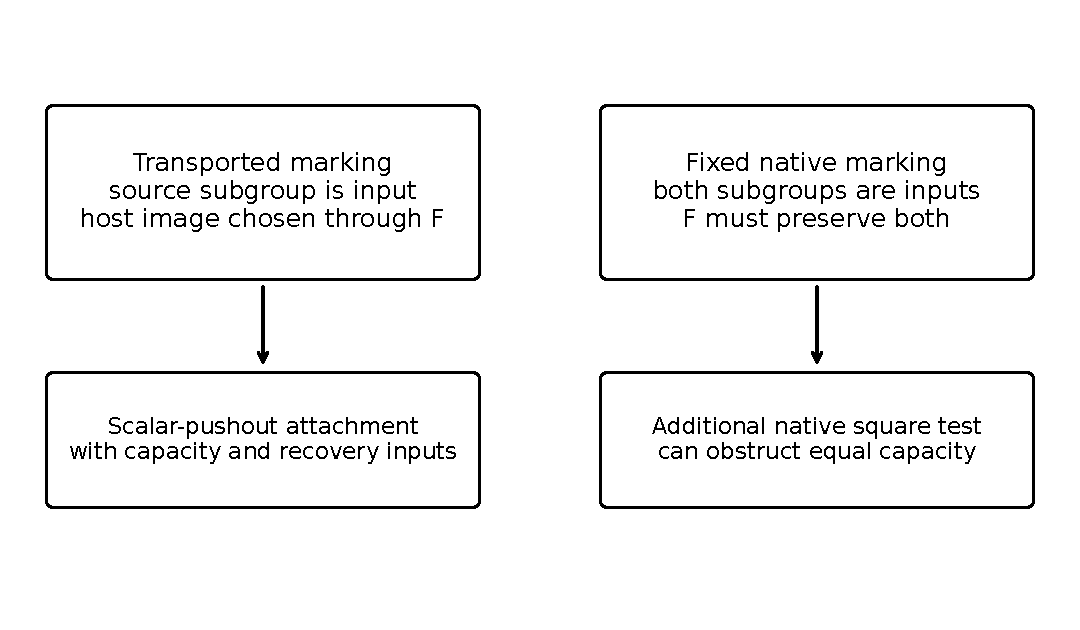
\includegraphics[width=\linewidth]{figures/V22.pdf}\end{center}
In the transported-marking contract, the source marking is supplied. After a permitted symplectic embedding and scalar-extension isomorphism have been chosen, the host marking is their image. A homomorphism fixes the represented center and carries squares, products, and specified lifts together.

In the independently fixed native contract, the target finite subgroup and its refinement are already given. The comparison must hit that subgroup with its existing marking. A scalar rescaling that changes it may be disallowed.
\[
\text{choose a compatible target marking}
\quad\ne\quad
\text{match this prescribed target marking}.
\]
The restricted one-vertex, trivial-stabilizer attachment retains its actual-type, capacity, full-character, and recovery hypotheses. It should not acquire an extra native-marking premise merely because a stronger problem is also studied. Conversely, that positive theorem cannot certify the stronger problem without computing the additional datum. The two branches in the figure remain separate throughout the atlas.
\vfill\PlateSource{Contract comparison}{Part III, Sections 26.4 and 27.3}{68}
